\documentclass[12pt,a4paper]{report}
\usepackage[a4paper, margin=2.5cm]{geometry}  % Following HTW guidelines
\usepackage{graphicx}
\usepackage{float}
\usepackage{hyperref}
\usepackage{amsmath, amssymb}
\usepackage{listings}
\usepackage[backend=biber,style=ieee,sorting=nty]{biblatex}
\usepackage{csquotes}
\usepackage{algorithm}
\usepackage{algpseudocode}
\usepackage[utf8]{inputenc}
\usepackage{placeins}
\usepackage{float}
    
\addbibresource{references.bib}

% Document settings following HTW guidelines
\renewcommand{\baselinestretch}{1.5}  % 1.5 line spacing
\setlength{\parindent}{0pt}  % No paragraph indentation
\setlength{\parskip}{6pt}    % Paragraph spacing

\begin{document}
% Include the title page
\begin{titlepage}
    \centering
    \vspace*{1cm}
    % University logo at the top
    
\includegraphics[width=0.3\textwidth]{media/Logo_HTW_Berlin.eps}\par\vspace{1cm}
    
    % University name
    {\Large HTW Berlin\par}\vspace{0.5cm}
    
    % Thesis title
    {\Huge\bfseries Neurobiologisch inspirierte Steuerung eines Roboters\par}\vspace{0.5cm}
    
    % Thesis type and your name
    {\Large Bachelorarbeit\par}\vspace{0.5cm}
    {\Large Amr Eslim\par}\vspace{0.5cm}
    
    % Supervisors information
    {\Large Erstbetreuer: Prof. Dr. Jochen Kerdels\par}\vspace{0.3cm}
    {\Large Zweitbetreuer: Prof. Dr. Frank Bauernöppel\par}\vspace{0.8cm}
    
    % Snake robot image at the bottom
    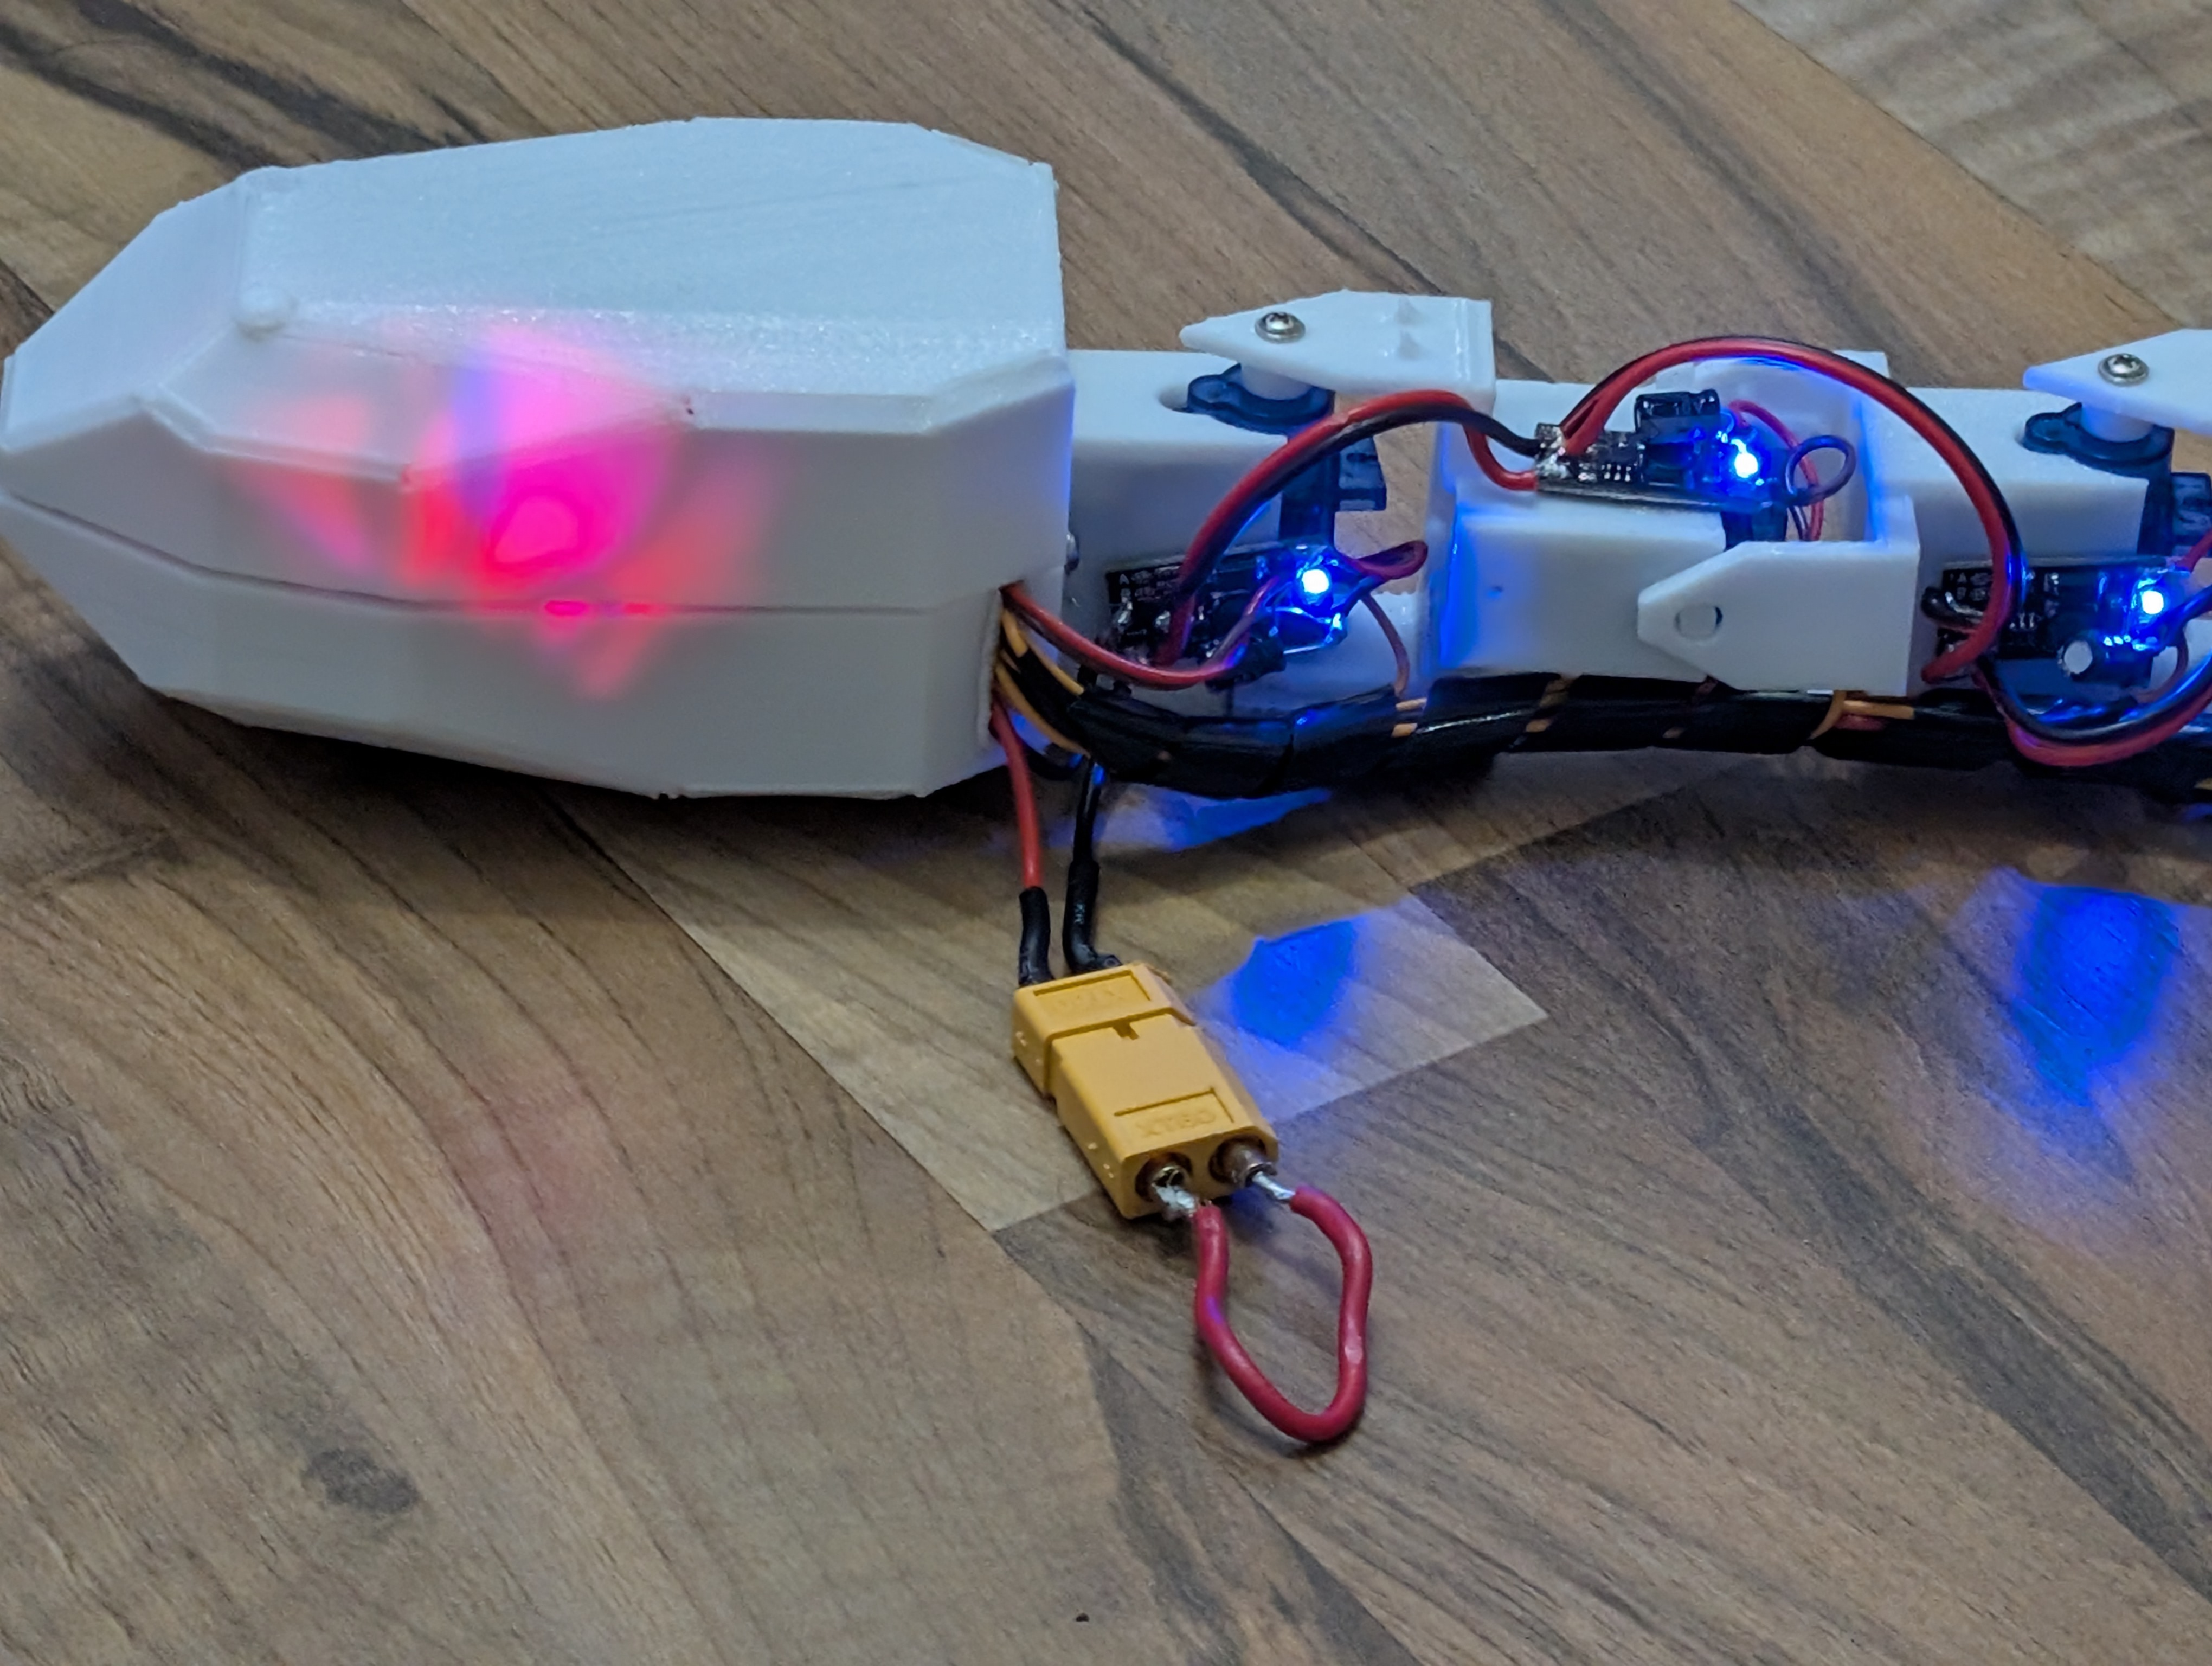
\includegraphics[width=0.3\textwidth]{media/snake_robot.jpg}\par\vspace{0.5cm}
    
    % Date (or submission details)
    {\Large \today\par}
\end{titlepage}






% Abstract
% \begin{abstract}
% This thesis presents the development and implementation of a bio-inspired snake robot, focusing on the integration of biological locomotion principles with modern robotics. The project encompasses multiple design iterations, addressing both hardware challenges and control system development. Key contributions include the implementation of various locomotion algorithms inspired by real snake movement patterns, particularly focusing on lateral undulation and serpentine motion. The development process involved creating a modular design using servo motors for precise movement control, implementing a sophisticated control system using CPG (Central Pattern Generator) principles, and extensive testing across different terrain types. Results demonstrate successful implementation of bio-inspired locomotion patterns, with quantitative analysis of movement efficiency and adaptability across various surfaces. This work contributes to the field of bio-inspired robotics by providing detailed insights into the development process and practical implementation of snake-like locomotion mechanisms.
% \end{abstract}
% \begin{abstract}
% This thesis presents the development and implementation of a bio-inspired snake robot control system. The focus is on replicating natural snake locomotion patterns through a modular robotic platform. A key contribution is the implementation of Central Pattern Generator (CPG) based control algorithms that enable smooth, coordinated movement. The system integrates joystick control for manual operation while maintaining biologically-inspired motion patterns. Testing demonstrates successful implementation of lateral undulation and other snake-like movements across different surfaces.
% \end{abstract}

% Table of Contents
\tableofcontents
\listoffigures
\listoftables


\chapter{Introduction}

\section{Background and Motivation}
Snake robots have emerged as a promising technological innovation inspired by the locomotion mechanisms observed in biological snakes. These robots exhibit exceptional adaptability in navigating confined spaces and overcoming challenging terrains where conventional wheeled or legged robots struggle. Their unique ability to generate smooth and continuous movements makes them particularly suitable for applications such as search-and-rescue missions, pipeline inspection, and medical procedures requiring minimally invasive interventions \textcite{transeth-2009, Hirose2004}.

The fundamental advantage of snake-like robots lies in their ability to replicate the efficient and versatile locomotion strategies of real snakes. By leveraging undulatory movements, these robots can traverse irregular surfaces, maneuver through narrow gaps, and maintain stability on diverse terrain \textcite{Seeja2022}. The inspiration from biological systems, coupled with advances in robotic control, has led to significant progress in the field, paving the way for innovative robotic applications.

\section{Research Objectives}
This research aims to contribute to the development of bio-inspired snake robots by focusing on the following key objectives:

\begin{itemize}
    \item Design and construct a modular snake robot with multiple degrees of freedom to enable flexible and adaptive movement.
    \item Develop and optimize biologically inspired control algorithms to achieve efficient and stable locomotion.
    \item Implement and evaluate different motion patterns, including lateral undulation and serpentine locomotion, to enhance adaptability across various environments.
    \item Analyze the robot's performance metrics across different terrain types to assess its effectiveness and versatility.
    \item Integrate a robust hardware and software control system to ensure reliable operation and real-time adaptability in dynamic conditions.
\end{itemize}


\section{Thesis Structure}

This thesis is structured into multiple chapters, each covering a key aspect of the development and control of a bio-inspired snake robot. The chapters are organized as follows:

\paragraph{Chapter 1: Introduction} 
This chapter provides an overview of the research background, motivation, and objectives. It introduces the concept of neurobiologically inspired control in robotics, emphasizing the importance of Central Pattern Generators (CPGs) for snake-like locomotion. The scope, research questions, and structure of the thesis are also outlined.

\paragraph{Chapter 2: State of the Art} 
This chapter reviews the biological principles of snake locomotion, including natural movement patterns and biomechanics. It also explores the historical development and current state of snake robot research, covering simulation and modeling approaches, biologically inspired robotic designs, and neurological models for locomotion control. Special focus is given to the mathematical representation of CPG networks.

\paragraph{Chapter 3: System Design, Implementation, and Details} 
This chapter describes the hardware architecture, including mechanical design using Onshape, 3D printing, and integration of the ESP32 microcontroller with 10 servo motors. The electronic architecture, control system configuration, WiFi-based communication, and core control parameters are detailed. It also discusses the implementation of movement algorithms such as lateral undulation and sidewinding.

\paragraph{Chapter 4: Experimental Results and Analysis} 
This chapter presents the performance evaluation of the snake robot. It includes detailed analyses of movement efficiency, optimization of control parameters, and testing under different environmental conditions. Specific evaluations include motion pattern analysis, power consumption, WiFi communication performance, endurance testing, and failure mode analysis.

\paragraph{Chapter 5: Conclusion and Future Work} 
The final chapter summarizes the research findings and contributions. It discusses the limitations of the current implementation and suggests directions for future improvements, including enhanced mechanical design, advanced control algorithms, and extended applications.

\paragraph{Appendices} 
Several appendices provide supporting documentation, including:
- Hardware documentation covering mechanical design, electronic components, and power systems.
- Software documentation detailing the system architecture, control software, and WiFi/web interface implementation.
- Experimental data, including testing protocols, environmental testing results, power consumption analysis, and control response evaluations.

\chapter{State of the Art}

\section{Biological Snake Locomotion}
Snake locomotion has been extensively studied as a foundation for bio-inspired robotics. According to \textcite{liljeback-2013}, snake motion can be characterized by several distinct patterns, each optimized for different environmental conditions and objectives. These patterns have been widely implemented in robotic systems to improve their adaptability and efficiency in traversing complex environments.

\textcite{liljeback-2013} present a fundamental analysis of lateral undulation, emphasizing its role in snake robots' ability to navigate diverse terrains efficiently. Further investigations have examined the biomechanical principles underlying these motion patterns, contributing to the development of advanced control strategies \textcite{lamping-2022}.

\subsection{Natural Snake Movement Patterns}
The primary motion patterns observed in biological snakes include:

\subsubsection{Lateral Undulation}
Lateral undulation, also known as serpentine motion, is the most common form of snake locomotion \textcite{liljeback-2013}. In this pattern, the snake creates a series of smooth curves that propagate from head to tail, generating forward thrust through the interaction with ground irregularities. \textcite{liljeback-2013} describe this as a wave-like motion where the snake's body follows the path traced by its head, with each segment of the body following the same spatial curve but with a time delay. 

\subsubsection{Rectilinear Motion}
Based on \textcite{Zhenli2006} rectilinear locomotion occurs when "the skin of the ventral surface is moved forward and backward by strong muscles and the broad belly scales grip the ground, moving the snake forward in a straight line." The authors note that this form of locomotion "is used only by the heavier-bodied snakes."

\subsubsection{Sidewinding}
Sidewinding is "probably the most astonishing gait to observe and is mostly used by snakes in the desert" \textcite{transeth-2009}. During this locomotion, "the snake lifts and curves its body leaving short, parallel marks on the ground while moving at an inclined angle" \textcite{transeth-2009}. Unlike other gaits like lateral undulation, sidewinding involves "brief static contact between the body of the snake and the ground" \textcite{transeth-2009}. This movement pattern is particularly useful "on surfaces with low shear such as sand" where snakes can achieve velocities up to 3 km/h \textcite{transeth-2009}.

\subsection{Biomechanical Principles}
The effectiveness of snake locomotion relies on several key physical principles:

\subsubsection{Friction Models}
As \textcite{lamping-2022} thoroughly analyze, anisotropic friction is crucial for effective snake movement. The contrast in forward versus reverse friction coefficients drives directional locomotion. This principle is significant for designing snake robots, which often require artificial scales or surface modifications to mimic this property. These mechanisms that enhance friction in snake-like robots are vital to improving their efficiency and ability to adapt to a wide range of surfaces.

\subsubsection{Propulsion Mechanics}
The generation of propulsive forces in snake locomotion is achieved through strategic interactions with environmental push-points, where reaction forces contribute to forward movement.\textcite{Bayraktaroglu2006} describe how a snake-like robot mimics natural lateral undulation by utilizing push-points in the environment. Each module follows its predecessor, ensuring coordinated motion, while the orientation of reaction forces determines the overall direction of movement. The applied motor control inputs facilitate continuous progression similar to biological snakes.
Additionally, rhythmic motion in biological and robotic systems is governed by central pattern generators (CPGs).\textcite{MARDER2001R986} explain that CPGs are neuronal circuits capable of producing rhythmic motor patterns such as walking, swimming, and flying without the need for sensory feedback. These circuits, found in both invertebrates and vertebrates, play a crucial role in coordinating motion patterns, with neuromodulatory pathways influencing their function. CPGs provide a robust framework for studying motor control mechanisms and their applications in robotic locomotion.

\section{Snake Robots: State of the Art}

\subsection{Historical Development}
The generation of propulsive forces in snake locomotion is achieved through strategic interactions with environmental push-points, where reaction forces contribute to forward movement. Bayraktaroglu et al. (2006) describe how a snake-like robot mimics natural lateral undulation by utilizing push-points in the environment. Each module follows its predecessor, ensuring coordinated motion, while the orientation of reaction forces determines the overall direction of movement. The applied motor control inputs facilitate continuous progression similar to biological snakes \textcite{Bayraktaroglu2006}.

Additionally, rhythmic motion in biological and robotic systems is governed by central pattern generators (CPGs). Marder and Bucher (2001) explain that CPGs are neuronal circuits capable of producing rhythmic motor patterns such as walking, swimming, and flying without the need for sensory feedback. These circuits, found in both invertebrates and vertebrates, play a crucial role in coordinating motion patterns, with neuromodulatory pathways influencing their function. CPGs provide a robust framework for studying motor control mechanisms and their applications in robotic locomotion \textcite{MARDER2001R986}.


\subsection{Current Research Directions}
Contemporary research in snake robotics is focused on enhancing locomotion efficiency, adaptability, and control mechanisms. Several key areas of investigation include:

\subsubsection{Control Systems}
Central Pattern Generators (CPGs) have emerged as a powerful tool for generating rhythmic movements in snake robots.
\textcite{Seeja2022} discuss the application of Central Pattern Generator (CPG) algorithms in snake-like robot locomotion, particularly to avoid obstacles. The study highlights that CPG models enable the robot to adjust its trajectory dynamically, allowing it to turn and evade obstacles. In addition, the incorporation of sensory feedback enhances collision detection. The research also introduces a phase transition method that utilizes phase-difference control parameters to facilitate smooth turning motions. This neural oscillator-based CPG approach is employed to generate rhythmic locomotion patterns, including rectilinear and lateral undulation gaits.

\subsubsection{Alternative Locomotion Strategies}
\textcite{yamano-2023} propose a rolling motion strategy for snake-like robots that enhances efficiency by utilizing a shift in the center of gravity (COG). Their approach divides the rolling motion into four distinct phases: (1) the kick stage, where the robot’s head or tail moves to initiate ground contact and generate rolling motion; (2) COG shift stage I, in which a heavier link at the head or tail moves forward to reposition the COG; (3) COG shift stage II, where the same link is raised to further adjust the COG; and (4) the rolling stage, where gravity facilitates continuous rolling motion.

\subsubsection{Mechanical Design and Adaptability}
The impact of mechanical parameters, particularly scale angles and friction coefficients, on the locomotion of snake robots has been extensively studied. Research by \textcite{shen-2021} demonstrated that the angle of the robot’s scales can be dynamically adjusted using air pressure, directly influencing its movement efficiency. Their experiments revealed that an optimal anchoring coefficient is achieved when the scale angle is around 26.7° at a pressure of 12 kPa, significantly improving forward propulsion. Conversely, when the pressure exceeds 22 kPa, the scales flip direction, enabling backward locomotion. This adaptive approach mimics biological snake adaptations by altering surface friction to enhance traction and maneuverability.

\subsection{Simulation and Modeling}
Accurate modeling is essential for designing and optimizing snake robot locomotion. \textcite{liljeback-2013} provide a foundational analysis of lateral undulation, introducing a simplified dynamic model for control design and stability analysis. Their study highlights that effective locomotion control must incorporate time-varying strategies, as static control laws fail to stabilize the system due to its inherent dynamics. Using averaging theory, they derived fundamental relationships between gait parameters and forward velocity, showing that the robot’s motion can be analytically predicted and optimized based on these parameters. This work has been instrumental in developing physics-based simulations that enable rapid prototyping and validation of locomotion strategies.

An additional contribution to simulation methodologies comes from \textcite{yogesh2023snake}, who provides open-source simulation tools for snake robot modeling. These practical implementations facilitate experimentation with different control strategies and locomotion patterns, supporting researchers in optimizing robot performance before physical deployment.

\subsection{Biologically Inspired Snake-like Robots}
Bio-inspired design principles continue to drive innovations in snake robotics. \textcite{Mohammed2016} developed a 3D printed modular snake robot that integrates flexible joint structures, enhancing both maneuverability and robustness. Their research highlights the benefits of modularity, where each module functions as a single rotational joint with one degree of freedom (DOF). The robot's structure allows for movement across multiple axes, enabling adaptability in various applications, such as search-and-rescue and medical robotics.

Building on this, \textcite{Arachchige2021} explored the potential of soft robotic snakes (SRS) by incorporating spatial bending capabilities to extend locomotion beyond conventional planar gaits. Their study demonstrates how continuous and smooth bending enables snake robots to better replicate biological movement, allowing for improved adaptability in climbing, swimming, and traversing complex terrains. These advancements highlight how soft robotics principles enhance maneuverability while maintaining structural integrity and operational efficiency.

\section{Neurological Models of Snake Locomotion}

The locomotion of snakes has been extensively studied, revealing that their movement is governed by a complex neural system that enables adaptive and rhythmic motion. This capability is primarily controlled by Central Pattern Generators (CPGs), which are neural circuits responsible for generating rhythmic outputs without requiring continuous sensory feedback. These circuits, located within the spinal cord, play a fundamental role in orchestrating rhythmic behaviors such as walking, swimming, and crawling in both vertebrates and invertebrates \textcite{MARDER2001R986}

\subsection{Biological Neural Control}

Biological snakes exhibit highly coordinated and adaptable movements, facilitated by a hierarchical neural control system. The spinal cord and peripheral nervous system function together to generate oscillatory patterns required for movement, even in the absence of sensory input. This suggests the existence of intrinsic neural oscillators that can sustain rhythmic activity autonomously \textcite{Inoue2007}. However, while CPGs can generate fundamental locomotor rhythms, sensory feedback plays a crucial role in modulating these patterns to refine motion and adapt to environmental variations \textcite{MARDER2001R986}.

Studies have shown that \textbf{proprioceptive and exteroceptive feedback} dynamically influence CPG activity, allowing for more stable and adaptive movement. This feedback mechanism enables snakes to transition between different locomotion patterns, such as \textbf{lateral undulation, concertina movement, and sidewinding}, depending on the terrain and external perturbations \textcite{Inoue2007}. Additionally, research on \textbf{CPG-based locomotion control in robotic snakes} has demonstrated that coupled neural oscillators can effectively reproduce these natural movements, allowing for continuous sinusoidal firing patterns in serpentine motion and controlled recovery periods for rectilinear movement  \textcite{manzoor-2019}.


\subsection{Central Pattern Generator (CPG) Model}
Central Pattern Generators (CPGs) are distributed neural networks that generate rhythmic motor outputs and are fundamental for biological locomotion. These networks have been extensively studied in the context of snake-like robot control, where they mimic the segmented structure of a real snake. Typically, CPG models consist of coupled oscillators arranged in a chain-like formation, producing phase-shifted rhythmic signals that facilitate coordinated joint actuation \textcite{wang2020cpg}.

Research has demonstrated that a simulated snake-like robot controlled by a CPG network can dynamically adapt to varying ground friction conditions through proprioceptive sensory feedback. In one study, friction sensors installed at the joints provided real-time input to sensory interneurons (SINs), allowing the system to adjust locomotion patterns accordingly. By processing frictional data through a combination of first-order lag and dead-time components, the robot was able to alter its movement in response to surface changes, improving stability and energy efficiency\textcite{Inoue2007}. 

Furthermore, a bidirectional cyclic inhibitory CPG model has been proposed to enhance locomotion adaptability. This model allows a snake-like robot to transition smoothly between different locomotion gaits—such as serpentine, concertina, and sidewinding—by incorporating feedback mechanisms from both higher-level neural control and environmental interactions\textcite{Zhenli2006}. 

Another approach involves a cyclic inhibitory CPG network designed specifically for 3D locomotion. Simulations conducted using a dynamic model in ADAMS software demonstrated that the robot could effectively navigate varying terrain by adjusting its joint oscillations and frictional response. The study highlighted the role of Coulomb friction in defining environmental interactions, which in turn influenced the adaptation strategy of the CPG-based control system\textcite{Lu2006}. 

These findings reinforce the effectiveness of CPG networks in controlling rhythmic, adaptive locomotion in snake-like robots. By integrating real-time sensory feedback and bidirectional neural inhibition, these models enable autonomous adaptation to environmental changes, thereby improving both stability and movement efficiency.

\subsection{CPG Modeling Approaches}

Several approaches have been proposed for modeling CPG-based control of snake-like robots. These can be broadly classified into the following categories:

\subsubsection{Mutual Inhibitory CPGs}

One of the fundamental architectures for generating rhythmic motion is the mutual inhibitory CPG model, which consists of neuron pairs that reciprocally inhibit each other, leading to stable oscillations. This architecture ensures continuous rhythmic movement. However, it lacks adaptability to environmental variations because it does not inherently produce sustained oscillations without additional adaptation mechanisms \textcite{Lu2006}.

\subsubsection{Cyclic Inhibitory CPGs}

Cyclic inhibitory CPG models address the limitations of mutual inhibitory architectures by incorporating feedback loops that enable the system to maintain oscillatory activity over time. These models involve interconnected neurons in a cyclic inhibitory structure, allowing for sustained and coordinated oscillations. This design proves particularly effective in generating stable 3D locomotion, as it enhances phase synchronization across multiple joints. Studies have demonstrated the effectiveness of this model in achieving robust serpentine motion, making it a preferable choice for controlling the locomotion of snake-like robots \textcite{Lu2006}.

\subsubsection{Sensory Feedback-Integrated CPGs}
Recent advancements in CPG modeling incorporate sensory feedback mechanisms, allowing adaptive locomotion. These models integrate sensory information through sensory interneurons (SIN), which relay environmental data back to the CPG, enabling real-time adjustments to oscillatory parameters \textcite{Inoue2007}. For instance, \textcite{Inoue2007} implemented a CPG-based control system where sensory input was processed by SIN and fed back into the CPG, enhancing the robot's ability to adapt to variations in ground friction.

\subsubsection{Evolutionary and Learning-Based CPGs}
Machine learning and evolutionary algorithms have been applied to optimize CPG parameters for snake locomotion. By employing genetic algorithms (GA), researchers have enabled robots to autonomously refine their locomotion patterns in response to different terrains and obstacles \textcite{Inoue2007}. Specifically, \textcite{Inoue2007} used GA to evolve CPG parameters that maximize adaptability across varying friction conditions, demonstrating that multi-environment performance-based evaluation functions enhance adaptive locomotion.

\subsection{Implementation Considerations}
When implementing CPG-based control, several key factors must be considered:
\begin{itemize}
    \item Phase Relationships Between Segments: To achieve effective serpentine locomotion, it is essential to maintain a consistent phase difference between joint oscillations. This phase control ensures synchronized movement, allowing the robot to generate propulsion force through interactions with the ground\textcite{Norzalilah2014}.
    \item Coupling Strengths Between Oscillators: The coordination between different segments of a CPG network is influenced by the strength of the connections between oscillators. Proper tuning of descending and ascending coupling pathways is necessary to ensure segmental synchronization, which requires detailed anatomical and electrophysiological studies\textcite{MARDER2001R986}.
    \item Adaptation Mechanisms for Environmental Feedback: A robust CPG-based system must integrate sensory feedback to adapt to environmental variations. Sensory inputs, such as ground reaction forces or muscle length changes, can be fed back into the CPG network to enhance stability and improve locomotion resilience against disturbances\textcite{Inoue2007}.
    \item Stability of Rhythm Generation: The stability of rhythmic motion depends on ensuring bounded and well-defined oscillatory behavior. Mathematical conditions such as Lipschitz continuity help establish the existence and uniqueness of stable rhythmic solutions in CPG models, preventing disruptions in locomotion patterns\textcite{Zhenli2006}.
\end{itemize}

These models provide a foundation for developing bio-inspired control systems that can generate smooth, coordinated motion patterns while maintaining adaptability to environmental changes.

\subsection{Mathematical Representation of CPG Networks}

The neural control system of a snake-like robot can be mathematically modeled as a network of coupled oscillators. As described by \textcite{wang2020cpg}. each oscillator in the network represents a segmental neural circuit. The system is structured as a single-chain bidirectional coupling network, where each connection between oscillators is defined by a phase lag parameter. The network's dynamics are governed by the following set of differential equations:

\begin{equation}
    \dot{\theta}_k =
    \begin{cases} 
        2\pi v + w \sin(\theta_2 - \theta_1 + \phi), & k = 1 \\
        2\pi v + w \left[\sin(\theta_{k-1} - \theta_k - \phi) + \sin(\theta_{k+1} - \theta_k + \phi)\right], & 2 \leq k \leq N-1 \\
        2\pi v + w \sin(\theta_{N-1} - \theta_N - \phi), & k = N
    \end{cases}
\end{equation}

where \( \theta_k \) represents the phase of the \( k \)-th oscillator, \( v \) denotes the intrinsic oscillation frequency, and \( w \) is the coupling strength between oscillators. The output of each oscillator, corresponding to the joint angle in a snake-like robot, is given by:

\begin{equation}
    \phi_k = A \cos(\theta_k), \quad 1 \leq k \leq N
\end{equation}

where \( A \) represents the oscillation amplitude. This mathematical formulation provides a precise method for generating rhythmic movement, crucial for implementing bio-inspired locomotion strategies in snake-like robots \textcite{wang2020cpg}.


%//////////////////////////////////////
%//////////////////////////////////////
%//////////////////////////////////////
%//////////////////////////////////////
%//////////////////////////////////////

\chapter{System Design, Implementation, and Details}

This chapter presents the complete design and implementation of the bio-inspired snake robot system. The design draws inspiration from biological snake locomotion patterns \cite{transeth-2009} and implements Central Pattern Generator (CPG) based control strategies similar to those discussed by \cite{Inoue2007}. The system architecture encompasses hardware design, control implementation, and motion pattern generation, with a focus on achieving versatile locomotion modes through a modular approach.

\section{Evolution of System Design}
The development of the snake robot proceeded through multiple iterations, each addressing specific challenges and limitations identified during testing and implementation.

\subsection{Initial Prototype}
The first iteration of the snake robot utilized an STM32-L432KC microcontroller with the following configuration:
\begin{itemize}
    \item Control Unit: STM32-L432KC microcontroller
    \item Power Supply: 3.7V Li-ion battery (18650)
    \item Voltage Regulation: 3V to 5V buck converters
    \item Signal Processing: 8 and 4 channel level shifters
    \item Actuation: 10 Miuzei 9G micro servos
\end{itemize}

Initial testing revealed several limitations:
\begin{itemize}
    \item Limited motion control capabilities due to microcontroller constraints
    \item Mechanical instability in the single-point contact hinge design
    \item Restricted movement to horizontal plane only
    \item Complex wiring due to centralized power distribution
\end{itemize}

\subsection{Final System Architecture}
The improved design iteration addressed previous limitations through several key modifications:
\begin{itemize}
    \item Migration to ESP32 microcontroller for enhanced connectivity and processing capabilities
    \item Redesigned power distribution system with distributed buck converters
    \item Implementation of signal integrity improvements through capacitive filtering ($100\mu F$, 16V) and pull-down resistors ($10k\Omega$)
    \item Addition of current sensing capabilities using ACS712 sensor
    \item Integration of TPU-printed passive scales for improved ground interaction
\end{itemize}
    %/////////////////////////////////////////////////////////
    %/////////////////////////////////////////////////////////
    %/////////////////////////////////////////////////////////
    %/////////////////////////////////////////////////////////
\section{Hardware Implementation}
\subsection{Mechanical Design}
The mechanical structure implements a modular approach similar to that described by \cite{wang-2016}, with several key improvements for enhanced stability and motion capability.
\subsubsection{Segment Design}
Each segment of the snake robot consists of:
\begin{itemize}
    \item Servo motor holder with dual contact points for improved stability
    \item Integrated electronics bay for local power regulation
    \item TPU-printed passive scales for ground interaction
    \item Dual-axis joint mechanism enabling both horizontal and vertical motion

\end{itemize}
\subsubsection{Modular Component Design}
The snake robot's mechanical structure consists of four distinct types of 3D-printed modules, each designed to serve specific functions while maintaining overall system integration \cite{Mohammed2016}. 

\paragraph{Head Module}
The head module serves as the control center and power hub of the robot:
\begin{itemize}
    \item Houses the ESP32 microcontroller and primary power components
    \item Features an integrated 18650 battery compartment
    \item Contains the ACS712 current sensor mounting area
    % \item Includes ventilation slots for thermal management
    \item Incorporates cable routing channels for organized wire management
\end{itemize}

\paragraph{Horizontal Axis Modules}
These modules form the primary locomotion segments:
\begin{itemize}
    \item Dual-point servo mounting system for enhanced stability
    \item Integrated electronics bay for buck converter placement
    \item Reinforced connection points to handle lateral forces
    \item Cable management channels for power and signal wires
\end{itemize}

\paragraph{Vertical Axis Modules}
Specialized segments enabling three-dimensional motion:
\begin{itemize}
    \item Modified servo mounting orientation for vertical actuation
    \item Enhanced structural support for lifting forces
    \item Compatible connection points with horizontal modules
    % \item Integrated passive scale mounting points
\end{itemize}

\paragraph{Tail Module}
The terminal segment designed for:
\begin{itemize}
    % \item Weight distribution optimization
    % \item Cable strain relief
    % \item Protective electronics enclosure
    % \item Aerodynamic profile for reduced motion resistance
\end{itemize}

The servo layout follows a specific pattern to enable both lateral undulation and sidewinding motions:
\begin{lstlisting}[language=C++]
const int servoLayout[NUM_SERVOS] = {1,0,1,1,0,1,1,0,1,1};
// 1=horizontal, 0=vertical
\end{lstlisting}

This arrangement, inspired by the work of \cite{Seeja2022}, provides:
\begin{itemize}
    \item 7 horizontal servos for lateral movement and wave propagation
    \item 3 vertical servos for lifting and sidewinding capabilities
\end{itemize}

\subsection{Electronic System}
\subsubsection{Power Distribution}
The power system implements a distributed architecture:
\begin{itemize}
    \item Main power: Single 18650 Li-ion battery (3.7V)
    \item Local regulation: Individual buck converters for each servo
    \item Noise suppression: 100μF capacitors parallel to each buck converter
    \item Current monitoring: ACS712 sensor for power consumption analysis
\end{itemize}

\subsubsection{Signal Integrity}
Signal integrity improvements include:
\begin{itemize}
    \item 10kΩ pull-down resistors on all servo control lines
    %/////////////////////////////////////////////////////////
    %/////////////////////////////////////////////////////////
    %/////////////////////////////////////////////////////////
    %/////////////////////////////////////////////////////////
    \item Distributed ground plane design
    \item Short signal paths through modular design
    %/////////////////////////////////////////////////////////
    %/////////////////////////////////////////////////////////
    %/////////////////////////////////////////////////////////
    %/////////////////////////////////////////////////////////
\end{itemize}

\section{Control System Architecture}
\subsection{Core Control System}
The control system implements a bio-inspired approach based on Central Pattern Generators (CPGs) \cite{MARDER2001R986}, utilizing the ESP32's capabilities for both pattern generation and wireless control.The system architecture consists of:
\begin{itemize}
    \item Motion pattern generator for servo control
    \item Web server for remote parameter adjustment
    \item Real-time parameter update system
    \item Current monitoring and data logging
\end{itemize}


\subsubsection{Motion Control Parameters}
The system uses the following key parameters for motion control:

\begin{lstlisting}[language=C++]
// Motion Parameters
float amplitude = 30.0;      // Wave amplitude (degrees)
float frequency = 1.0;       // Oscillation frequency (Hz)
float phaseOffset = 60.0;    // Phase offset between segments
float centerPosition = 90.0; // Neutral position (degrees)
\end{lstlisting}
Parameter constraints are implemented to ensure mechanical safety:
\begin{itemize}
    \item Amplitude: Limited to 10-45 degrees
    \item Frequency: Range of 0.1-2.0 Hz
    \item Phase offset: Constrained between 30-90 degrees
\end{itemize}

These parameters are dynamically adjustable through the web interface, allowing real-time motion pattern modification.

\subsection{Wireless Interface Implementation}
The ESP32 creates a wireless access point and web server for remote control:

\begin{lstlisting}[language=C++]
WiFi.softAP("ESP32_Snake", "12345678");
server.on("/", HTTP_GET, handleRoot);
server.on("/", HTTP_POST, handleSetParameters);
server.on("/current", HTTP_GET, handleCurrentData);  
server.on("/download", HTTP_GET, handleDownload);
\end{lstlisting}

The web interface provides:
\begin{itemize}
    \item Real-time parameter adjustment
    \item Movement mode selection
    \item System monitoring capabilities
    \item Diagnostic functions
\end{itemize}

Parameter updates are handled through HTTP POST requests:

\begin{lstlisting}[language=C++]
void handleSetParameters() {
    if (server.hasArg("amplitude")) {
        amplitude = constrain(server.arg("amplitude").toFloat(), 
                            10.0, 45.0);
    }
    // Similar handlers for frequency and phase
}
\end{lstlisting}

\section{Motion Pattern Generation}
\subsection{Lateral Undulation}
The lateral undulation pattern, based on the work of \cite{liljeback-2013}, is implemented as a traveling wave:

\begin{equation}
\theta_i(t) = A \sin(\omega t + \phi_i) + \theta_{\text{offset}}
\end{equation}

Where:
\begin{itemize}
    \item $\theta_i(t)$ is the angle of the i-th servo at time t
    \item $A$ is the amplitude
    \item $\omega = 2\pi f$ is the angular frequency
    \item $\phi_i$ is the phase offset for segment i
    \item $\theta_{\text{offset}}$ is the center position
\end{itemize}

The implementation includes direction control:

\begin{lstlisting}[language=C++]
void updateServosLateralUndulation() {
    float timeScale = millis() * 0.001 * frequency * 2 * PI;
    int horizontalIndex = 0;
    
    for (int i = 0; i < NUM_SERVOS; i++) {
        if (servoLayout[i] == 1) {
            float phase = forwardDirection ? 
                radians(horizontalIndex * phaseOffset) : 
                radians((NUM_HORIZONTAL - 1 - horizontalIndex) * phaseOffset);
            float angle = centerPosition + amplitude * sin(timeScale + phase);
            servos[i].write(angle);
            horizontalIndex++;
        }
    }
}
\end{lstlisting}

\subsection{Sidewinding Implementation}
The sidewinding motion, inspired by \cite{yamano-2023}, combines horizontal and vertical waves with a phase offset:

\begin{lstlisting}[language=C++]
void updateServosSidewinding() {
    float timeScale = millis() * 0.001 * frequency * 2 * PI;
    for (int i = 0; i < NUM_SERVOS; i++) {
        if (servoLayout[i] == 1) {
            // Horizontal motion
            float angle = centerPosition + amplitude * 
                         sin(timeScale + horizontalPhase);
            servos[i].write(angle);
        } else {
            // Vertical motion with 90-degree phase offset
            float angle = centerPosition + verticalAmplitude * 
                         sin(timeScale + verticalPhase + PI/2);
            servos[i].write(angle);
        }
    }
}
\end{lstlisting}

\section{System Performance and Limitations}
\subsection{Performance Analysis}
Current system capabilities include:
\begin{itemize}
    \item Update rate: 50Hz (20ms interval)
    \item Wireless control range: approximately 50 meters
    \item Motion patterns: Lateral undulation and sidewinding
    \item Real-time parameter adjustment
\end{itemize}

\subsection{Current Limitations}
\begin{itemize}
    \item No closed-loop feedback for servo positions
    \item Limited battery life under continuous operation
    \item WiFi range constraints in certain environments
    \item Mechanical wear on servo gears during sustained operation
\end{itemize}

\subsection{Future Improvements}
Based on the current limitations, several potential improvements are identified:
\begin{itemize}
    \item Implementation of position feedback sensors
    \item Enhanced power management systems
    \item Additional motion patterns based on biological studies
    \item Improved mechanical durability through material selection
\end{itemize}


%//////////////////////////////////////
%//////////////////////////////////////
%//////////////////////////////////////
%//////////////////////////////////////
%//////////////////////////////////////
\chapter{Experimental Results and Analysis}

\section{Performance Metrics}
The system's performance was evaluated based on:
\begin{itemize}
    \item Response time between command input and servo actuation
    \item Accuracy of amplitude and frequency control
    \item Stability of WiFi connection during operation
    \item Battery life under continuous operation
\end{itemize}

\section{Control Parameter Optimization}
Through experimental testing, optimal parameters were determined:
\begin{itemize}
    \item Amplitude range: 20° - 45° for stable locomotion
    \item Frequency range: 0.5 - 2.0 Hz for efficient movement
    \item Update interval: 50ms for smooth motion
    \item Phase offset: $\pi/2$ between adjacent segments
\end{itemize}

\section{System Limitations}
Current implementation limitations include:
\begin{itemize}
    \item WiFi connectivity and response time
    \item Maximum of 16 servo motors due to ESP32 GPIO limitations
    \item Update rate constrained by WebServer handling capacity
    \item Battery life affected by continuous WiFi operation and the high demand of the servos
\end{itemize}

% Appendices
\appendix
%//////////////////////////////////////
%//////////////////////////////////////
%//////////////////////////////////////
%//////////////////////////////////////
%//////////////////////////////////////
\chapter{Hardware Specifications}
\section{Mechanical Design}
\subsection{3D Printed Components}
%//////////////////////////////////////
%//////////////////////////////////////
%//////////////////////////////////////
The robotic system comprises several 3D-printed parts designed for structural integrity, modularity, and functionality. Below are the primary components:
\FloatBarrier
\subsubsection{Head Assembly}

The head is split into two sections: \textbf{top-head} and \textbf{bottom-head}, which encase sensors and other electronics.

\begin{itemize}
\item Material: PETG
\item Print Settings: 0.2mm layer height, 30\%  gyroid infill
\item Features:
\begin{itemize}
% \item Eye placeholders for sensors
\item Reinforced mounting slots
\item Structured surface for aesthetics and strength
\end{itemize}
\end{itemize}
\begin{figure}[h]
\centering
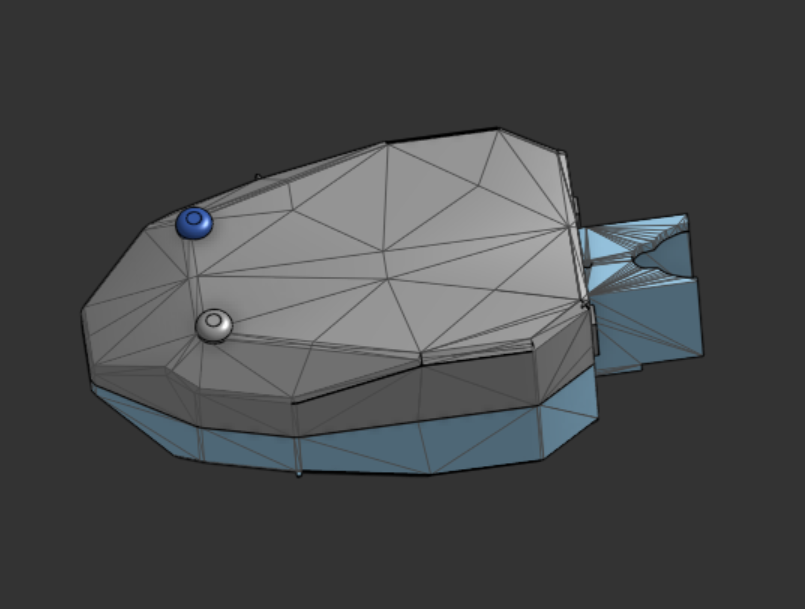
\includegraphics[width=0.5\textwidth]{media/Head.png}
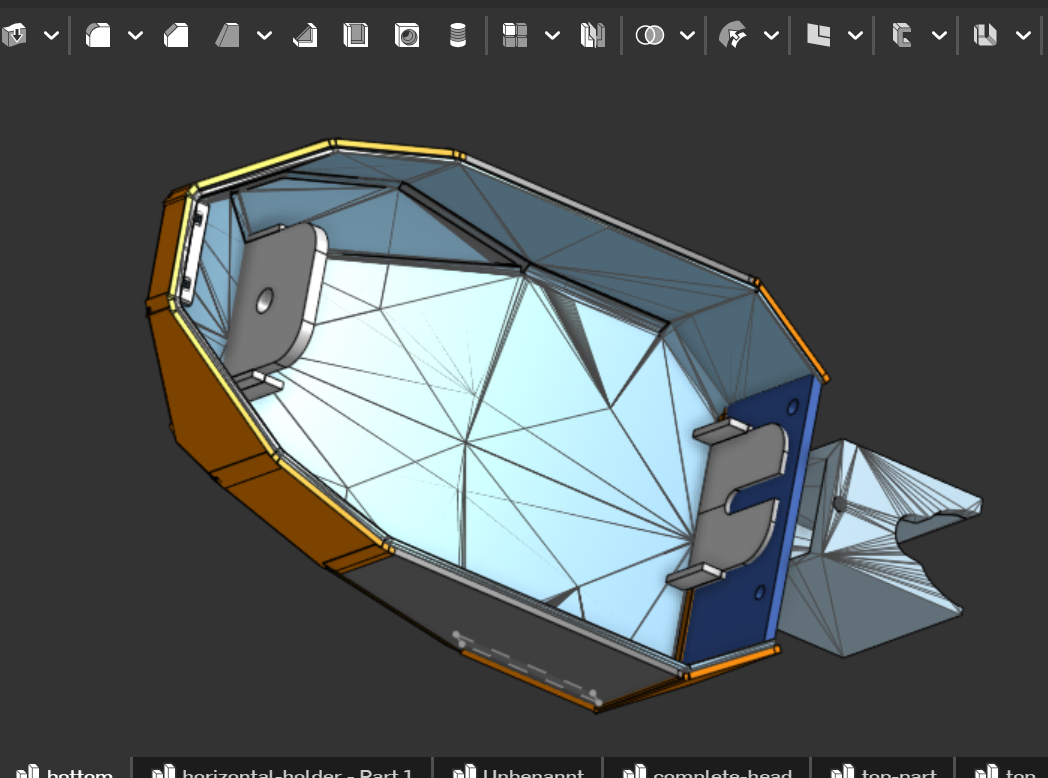
\includegraphics[width=0.5\textwidth]{media/Bottom-Head.png}
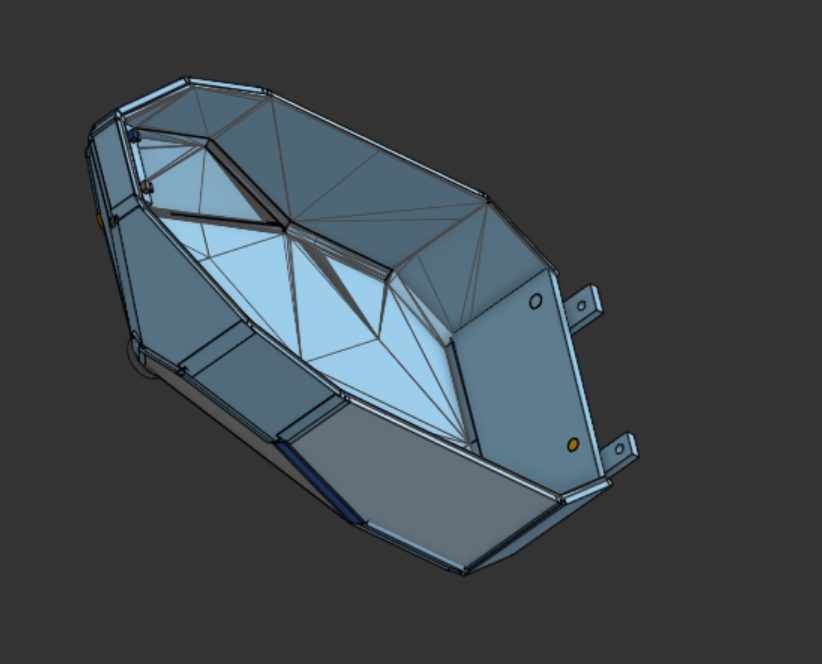
\includegraphics[width=0.5\textwidth]{media/top-head.png}
\caption{Top and bottom head assembly}
\end{figure}

\FloatBarrier
\subsubsection{Tail Structure}

The \textbf{tail-part} connects the main body to the rear stabilizers and allows controlled movement.

\begin{itemize}
\item Material: PETG
\item Print Settings: 0.2mm layer height, 25% infill
\item Features:
\begin{itemize}
\item Reinforced mounting points for servos
\item Aerodynamic design
\item Cable routing slots
\end{itemize}
\end{itemize}
\begin{figure}[h]
\centering
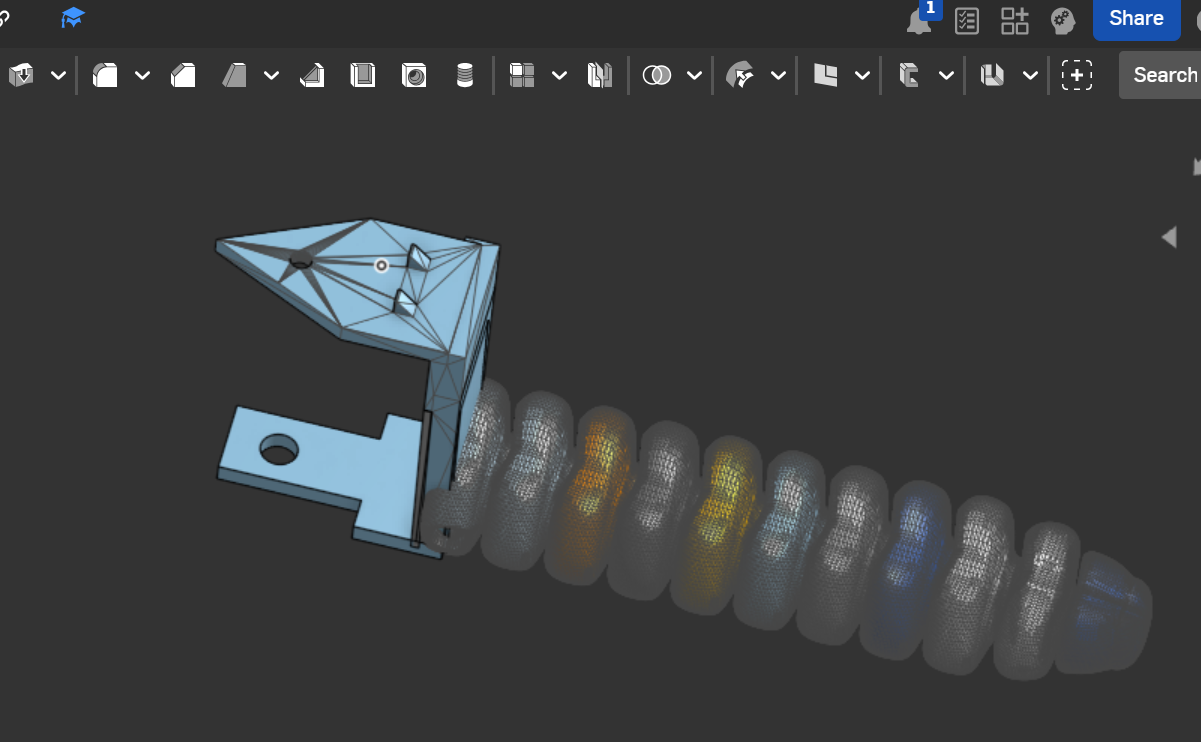
\includegraphics[width=0.5\textwidth]{media/Tail-part.png}
\caption{tail-part assembly}
\end{figure}

\FloatBarrier
\subsubsection{Scales for Friction Optimization}

The \textbf{scales-scaled} part consists of an array of overlapping scales designed to improve friction control during movement.

\begin{itemize}
\item Material: PETG
\item Print Settings: 0.15mm layer height for fine details
\item Features:
\begin{itemize}
\item Lightweight yet strong design
\item Flexible attachment points
\item Surface texture optimized for traction
\end{itemize}
\end{itemize}
\begin{figure}[h]
\centering
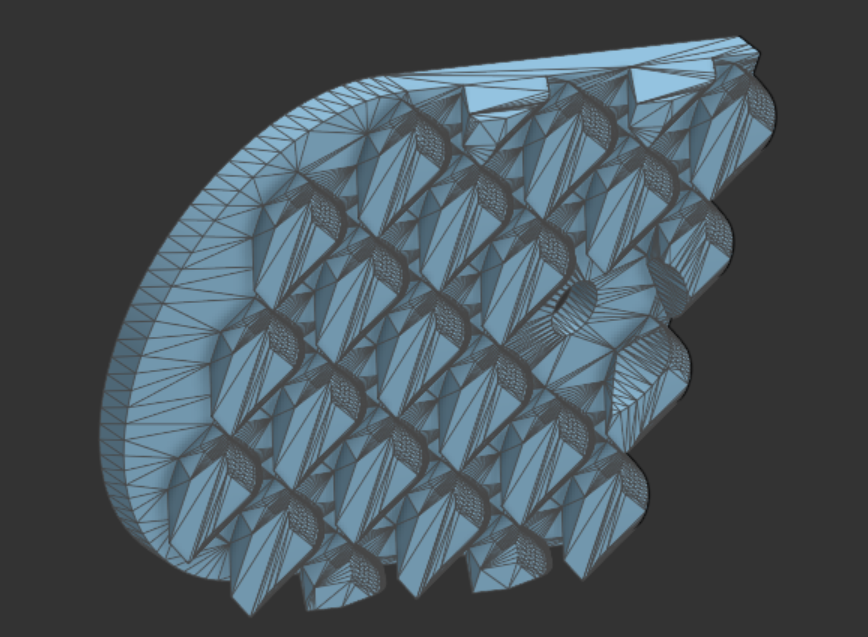
\includegraphics[width=0.5\textwidth]{media/scales.png}
\caption{3D printed scales for movement enhancement}
\end{figure}

\FloatBarrier
\subsubsection{Servo Holders}

Two types of servo mounts are used: \textbf{horizontal-holder} and \textbf{vertical-holder}, ensuring flexibility in positioning.

\begin{itemize}
\item Material: PETG
\item Print Settings: 0.2mm layer height, 40% infill for strength
\item Features:
\begin{itemize}
\item Snap-fit design for easy installation
\item Integrated cable management slots
\item Reinforced screw holes for secure mounting
\end{itemize}m
\end{itemize}

\begin{figure}[h]
\centering
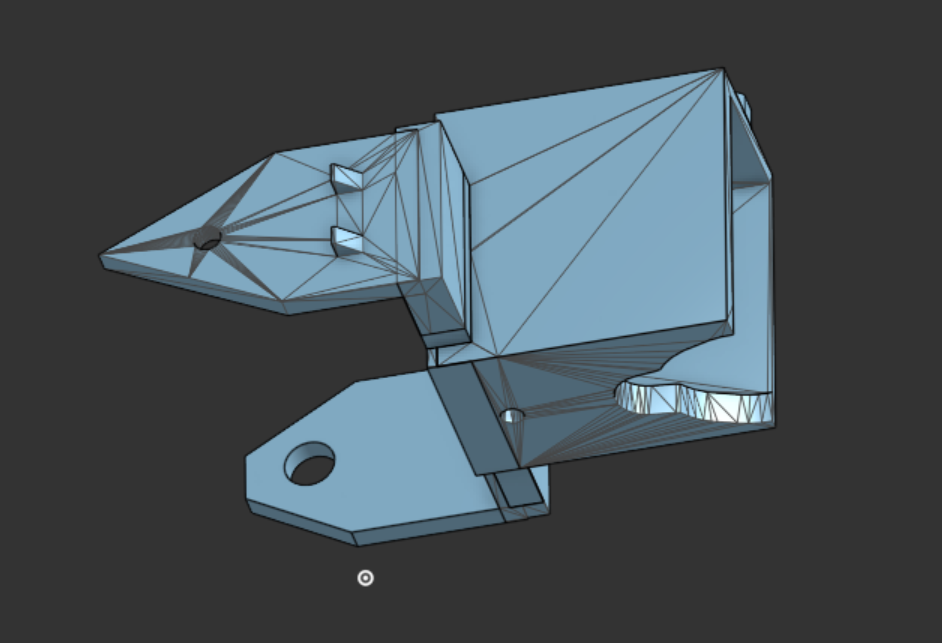
\includegraphics[width=0.5\textwidth]{media/Vertical-holder.png}
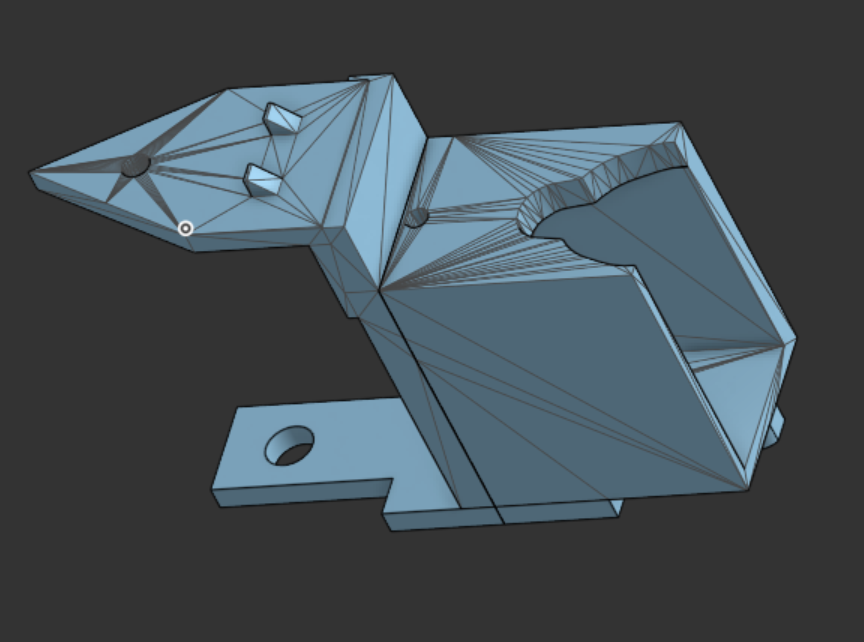
\includegraphics[width=0.5\textwidth]{media/Horizontal-holder.png}
\caption{Horizontal and Vertical servo holder}
\end{figure}

These components work together to form a bio-inspired robotic system with optimized movement and structural robustness.
%//////////////////////////////////////
%//////////////////////////////////////
\subsubsection{Main Body Segments}
\begin{itemize}
\item Primary segment specifications:
\begin{itemize}
\item Dimensions: 40mm x 40mm x 65mm (height x width x length)
\item Wall thickness: 2mm primary walls, 3mm reinforced areas
\item Infill: 30% gyroid pattern for optimal strength/weight ratio
\item Layer height: 0.2mm for good surface finish and strength
\item Material: PETG filament (eSun PETG+ or equivalent)
\item Print orientation: Vertical with supports for servo mounts
\item Print temperature: 235°C nozzle, 80°C bed
\item Print speed: 50mm/s outer walls, 80mm/s infill
\end{itemize}
\item Structural features:
\begin{itemize}
    \item Integrated cable routing channels (8mm diameter)
    \item M3 brass heat-set insert mounting points (x4 per servo)
    \item Snap-fit segment connectors with 0.2mm tolerance
    \item Reinforced corners with 1mm fillets
    \item Ventilation slots for servo cooling
\end{itemize}
\end{itemize}
\subsubsection{Electronics Housing}
\begin{itemize}
\item ESP32 mounting bay:
\begin{itemize}
\item Dimensions: 60mm x 40mm x 30mm
\item Mounting posts for M2.5 screws
\item Ventilation mesh pattern
\item Access ports for USB programming
\end{itemize}
\item Battery compartment:
\begin{itemize}
    \item 2S LiPo battery slot (75mm x 35mm x 20mm)
    \item Quick-release mechanism
    \item Strain relief for power cables
\end{itemize}
\end{itemize}
\section{Electronic Components}
\subsection{Microcontroller Specifications}
\begin{itemize}
\item ESP32-WROOM-32 Development Board:
\begin{itemize}
\item Dual-core Xtensa LX6 microprocessor
\item Operating frequency up to 240 MHz
\item 520 KB SRAM
\item 4 MB Flash memory
\item Integrated WiFi 802.11 b/g/n
\item Bluetooth 4.2 support
\item Operating voltage: 3.3V
\item 34x programmable GPIO pins
\end{itemize}
\end{itemize}
\subsection{Servo Motor Details}
\begin{table}[h]
\centering
\begin{tabular}{|l|l|}
\hline
\textbf{Parameter} & \textbf{Value} \\
\hline
Model & MG996R High Torque \\
Operating Voltage & 4.8V - 7.2V \\
Stall Torque (4.8V) & 9.4 kg$\cdot$cm \\
Stall Torque (6.0V) & 11 kg$\cdot$cm \\
Operating Speed (4.8V) & 0.17 sec/60$^{\circ}$ \\
Operating Speed (6.0V) & 0.14 sec/60$^{\circ}$ \\
Operating Angle & 180$^{\circ}$ $\pm$5$^{\circ}$ \\
Pulse Width Range & 500-2500 microseconds \\
Direction & Clockwise/Counter Clockwise \\
Dead Band Width & 1 microsecond \\
Temperature Range & -30$^{\circ}$C to +60$^{\circ}$C \\
Gear Type & Metal \\
Bearing Type & Dual Ball Bearing \\
Weight & 55g \\
Dimensions & 40.7 x 19.7 x 42.9 mm \\
\hline
\end{tabular}
\caption{Detailed Servo Motor Specifications}
\end{table}
\subsection{Power System}
\begin{itemize}
\item Battery:
\begin{itemize}
\item Type: 2S LiPo
\item Capacity: 2200mAh
\item Voltage: 7.4V nominal
\item C-Rating: 25C continuous
\item Weight: 135g
\end{itemize}
\item Power Distribution:
\begin{itemize}
    \item Custom PCB power distribution board
    \item 5V voltage regulator for ESP32
    \item Direct 7.4V supply for servos
    \item Current monitoring shunt resistor
    \item Power switch with LED indicator
    \item Low voltage cutoff at 6.6V
\end{itemize}
\end{itemize}   
%//////////////////////////////////////
%//////////////////////////////////////
%//////////////////////////////////////
%//////////////////////////////////////
%//////////////////////////////////////
\chapter{Software Documentation}

\section{System Architecture Overview}
The snake robot's control software is implemented on an ESP32 microcontroller using the Arduino IDE. The system integrates multiple components for comprehensive robot control, including servo motor control, wireless communication, locomotion pattern generation, and real-time monitoring capabilities.

\section{Core Implementation}
\subsection{System Configuration}
The fundamental configuration defines the robot's physical structure and control parameters:

\begin{lstlisting}[language=C++]
// Servo configuration
const int NUM_SERVOS = 10;
const int NUM_HORIZONTAL = 7;  // Number of horizontal servos
const int servoLayout[NUM_SERVOS] = {1, 0, 1, 1, 0, 1, 1, 0, 1, 1}; 
// 1=horizontal, 0=vertical
const int servoPins[NUM_SERVOS] = {23, 22, 2, 4, 16, 17, 5, 18, 19, 21};

// Motion control parameters
float amplitude = 30.0;      // Degrees
float frequency = 1.0;       // Hz
float phaseOffset = 60.0;    // Degrees
float centerPosition = 90.0; // Degrees
float verticalAmplitude = 20.0;  // For sidewinding
float verticalPhaseOffset = 90.0; // Degrees
\end{lstlisting}

\subsection{Motion Control System}
The software implements two primary locomotion patterns: lateral undulation and sidewinding. These patterns are implemented through specialized functions that calculate servo positions based on sinusoidal wave propagation.

\subsubsection{Lateral Undulation}
The lateral undulation pattern, typical for snake locomotion on flat surfaces:

\begin{lstlisting}[language=C++]
void updateServosLateralUndulation() {
    float timeScale = millis() * 0.001 * frequency * 2 * PI;
    int horizontalIndex = 0;
    
    for (int i = 0; i < NUM_SERVOS; i++) {
        if (servoLayout[i] == 1) {  // Horizontal servos
            float segmentPhase = horizontalIndex * 
                               radians(phaseOffset);
            
            if (!forwardDirection) {
                segmentPhase = (NUM_HORIZONTAL - 1 - horizontalIndex) * 
                             radians(phaseOffset);
            }
            
            float angle = centerPosition + 
                         amplitude * sin(timeScale + segmentPhase);
            servos[i].write(angle);
            horizontalIndex++;
        } else {  // Vertical servos
            servos[i].write(centerPosition);
        }
    }
}
\end{lstlisting}

\subsubsection{Sidewinding Motion}
The sidewinding pattern, which enables movement in more challenging terrains:

\begin{lstlisting}[language=C++]
void updateServosSidewinding() {
    float timeScale = millis() * 0.001 * frequency * 2 * PI;
    int horizontalIndex = 0;
    int verticalIndex = 0;

    for (int i = 0; i < NUM_SERVOS; i++) {
        if (servoLayout[i] == 1) {
            float phase = forwardDirection ? 
                radians(horizontalIndex * phaseOffset) : 
                radians((NUM_HORIZONTAL - 1 - horizontalIndex) * 
                phaseOffset);
            
            float angle = centerPosition + 
                         amplitude * sin(timeScale + phase);
            servos[i].write(angle);
            horizontalIndex++;
        } else {
            float phase = radians(verticalIndex * phaseOffset + 
                                verticalPhaseOffset);
            float angle = centerPosition + 
                         verticalAmplitude * sin(timeScale + phase);
            servos[i].write(angle);
            verticalIndex++;
        }
    }
}
\end{lstlisting}

\subsection{Network Communication}
The system creates a WiFi access point for remote control and implements a web server for user interaction:

\begin{lstlisting}[language=C++]
WiFi.softAP("ESP32_Snake", "12345678");
server.on("/", HTTP_GET, handleRoot);
server.on("/", HTTP_POST, handleSetParameters);
server.on("/current", HTTP_GET, handleCurrentData);
server.on("/download", HTTP_GET, handleDownload);
\end{lstlisting}

\subsection{Parameter Control System}
The implementation includes a flexible parameter control system that handles user inputs and maintains safe operating ranges:

\begin{lstlisting}[language=C++]
void handleSetParameters() {
    String response;
    
    if (server.hasArg("mode")) {
        movementMode = server.arg("mode").toInt();
    }
    
    if (server.hasArg("action")) {
        String action = server.arg("action");
        if (action == "forward") {
            locomotionEnabled = true;
            forwardDirection = true;
        } else if (action == "backward") {
            locomotionEnabled = true;
            forwardDirection = false;
        } else if (action == "stop") {
            locomotionEnabled = false;
            centerAllServos();
        }
    }

    if (server.hasArg("amplitude")) {
        amplitude = constrain(server.arg("amplitude").toFloat(), 
                            10.0, 45.0);
    }
    if (server.hasArg("frequency")) {
        frequency = constrain(server.arg("frequency").toFloat(), 
                            0.1, 2.0);
    }
    if (server.hasArg("phase")) {
        phaseOffset = constrain(server.arg("phase").toFloat(), 
                              30.0, 90.0);
    }
}
\end{lstlisting}

\subsection{Current Monitoring and Data Logging}
The system implements real-time current monitoring using an ACS712 sensor and logs data to the ESP32's SPIFFS filesystem:

\begin{lstlisting}[language=C++]
void handleCurrentData() {
    float current = 0.0;
    for(int i = 0; i < 10; i++) {
        current += abs(sensor.mA_DC());
        delay(1);
    }
    current = (current / 10.0) / 1000.0;  // Convert to Amps
    logCurrentData(current);
    
    String jsonResponse = "{\"current\": " + String(current, 3) + "}";
    server.send(200, "application/json", jsonResponse);
}

void logCurrentData(float current) {
    File file = SPIFFS.open("/current_log.txt", FILE_APPEND);
    unsigned long timestamp = millis();
    file.printf("%lu,%0.3f\n", timestamp, current);
    file.close();
}
\end{lstlisting}

\subsection{Main Control Loop}
The main loop coordinates all system functions:

\begin{lstlisting}[language=C++]
void loop() {
    server.handleClient();
    
    static unsigned long lastCheck = 0;
    if (millis() - lastCheck >= 60000) {
        checkLogFileSize();
        lastCheck = millis();
    }
    
    if (testingActive) {
        handleServoTest();
    }
    else if (locomotionEnabled && 
             (millis() - lastUpdate >= interval)) {
        if (movementMode == 0) {
            updateServosLateralUndulation();
        } else {
            updateServosSidewinding();
        }
        lastUpdate = millis();
    }
}
\end{lstlisting}

\section{Performance and Safety Features}
The implementation includes several key features for reliable operation:

\begin{itemize}
    \item 50Hz servo update rate for smooth motion
    \item Averaged current readings for improved accuracy
    \item Automatic file system management to prevent memory overflow
    \item Parameter constraints for stable operation
    \item Emergency stop functionality
    \item Non-blocking operations for responsive control
    \item Servo testing and calibration capabilities
\end{itemize}

\section{System Initialization}
The initialization process ensures proper setup of all components:

\begin{lstlisting}[language=C++]
void setup() {
    Serial.begin(115200);
    pinMode(analogPin, INPUT);
    analogReadResolution(12);
    
    if(!SPIFFS.begin(true)) {
        Serial.println("SPIFFS mount failed");
        return;
    }
    
    for (int i = 0; i < NUM_SERVOS; i++) {
        servos[i].attach(servoPins[i]);
        servos[i].write(centerPosition);
    }
    
    WiFi.softAP("ESP32_Snake", "12345678");
    
    server.on("/", HTTP_GET, handleRoot);
    server.on("/", HTTP_POST, handleSetParameters);
    server.on("/current", HTTP_GET, handleCurrentData);
    server.on("/download", HTTP_GET, handleDownload);
    server.begin();
}
\end{lstlisting}
%//////////////////////////////////////
%//////////////////////////////////////
%//////////////////////////////////////
%//////////////////////////////////////
%//////////////////////////////////////
\chapter{Test Data}
\section{Performance Testing Protocol}
\subsection{Motion Pattern Analysis}
\begin{enumerate}
\item \textbf{Linear Locomotion Tests}
\begin{itemize}
\item Course setup: 3-meter straight line with 10cm width markers
\item Starting position: Robot centered at start line
\item Test conditions:
\begin{itemize}
\item Amplitude variations: 20°, 30°, 40°
\item Frequency variations: 0.5Hz, 1.0Hz, 1.5Hz
\item Phase offset variations: 45°, 60°, 75°
\end{itemize}
\item Measurements:
\begin{itemize}
\item Time to complete course
\item Maximum lateral deviation
\item Power consumption
\item Servo temperature rise
\end{itemize}
\end{itemize}
\item \textbf{Turning Capability Tests}
\begin{itemize}
    \item Setup: 2-meter diameter circular test area
    \item Measurements:
    \begin{itemize}
        \item Minimum turning radius
        \item Time for 360° rotation
        \item Angular velocity
        \item Power consumption during turn
    \end{itemize}
    \item Variables:
    \begin{itemize}
        \item Different turn angles (45°, 90°, 180°)
        \item Various motion parameters
        \item Different surface types
    \end{itemize}
\end{itemize}
\end{enumerate}
\section{Environmental Testing}
\begin{table}[h]
\centering
\begin{tabular}{|l|c|c|c|}
\hline
\textbf{Surface Type} & \textbf{Friction Coef.} & \textbf{Speed (m/s)} & \textbf{Success Rate} \\
\hline
Smooth Tile & 0.3 & 0.15 & 95\% \\
Carpet & 0.6 & 0.08 & 85\% \\
Rubber Mat & 0.8 & 0.12 & 90\% \\
Concrete & 0.7 & 0.10 & 80\% \\
\hline
\end{tabular}
\caption{Surface Performance Characteristics}
\end{table}

\section{Power Consumption Analysis}
\begin{table}[h]
\centering
\begin{tabular}{|l|c|c|c|c|}
\hline
\textbf{State} & \textbf{Current (A)} & \textbf{Voltage (V)} & \textbf{Power (W)} & \textbf{Runtime (min)} \\
\hline
Idle & 0.2 & 7.4 & 1.48 & 660 \\
WiFi Only & 0.3 & 7.4 & 2.22 & 440 \\
Standby & 0.5 & 7.4 & 3.70 & 264 \\
Walking & 1.8 & 7.2 & 12.96 & 73 \\
Full Motion & 2.1 & 7.0 & 14.70 & 63 \\
\hline
\end{tabular}
\caption{Power Consumption in Different Operating Modes}
\end{table}
\section{WiFi Performance Metrics}
\begin{itemize}
\item Signal strength vs. distance measurements
\item Latency measurements at various distances
\item Packet loss analysis
\item Interface response times
\item Connection stability tests
\end{itemize}
\section{Detailed Test Results}


\subsection{Control Response Testing}
\begin{table}[h]
\centering
\begin{tabular}{|l|c|c|c|}
\hline
\textbf{Command} & \textbf{Response Time (ms)} & \textbf{Accuracy (\%)} & \textbf{Jitter (ms)} \\
\hline
Start Motion & 45 & 98 & $\pm$5 \\
Stop Motion & 38 & 99 & $\pm$3 \\
Change Direction & 52 & 95 & $\pm$7 \\
Parameter Update & 41 & 97 & $\pm$4 \\
\hline
\end{tabular}
\caption{Control System Response Metrics}
\end{table}

\subsection{Motion Pattern Analysis}
\begin{itemize}
\item \textbf{Lateral Undulation Tests}
\begin{table}[h]
\centering
\begin{tabular}{|c|c|c|c|c|}
\hline
\textbf{Amplitude ($^{\circ}$)} & \textbf{Frequency (Hz)} & \textbf{Speed (m/s)} & \textbf{Efficiency*} & \textbf{Stability**} \\
\hline
20 & 0.5 & 0.08 & 75\% & 90\% \\
30 & 1.0 & 0.12 & 85\% & 85\% \\
40 & 1.5 & 0.15 & 80\% & 75\% \\
\hline
\end{tabular}
\caption{Lateral Undulation Performance Data}
\end{table}
\small{* Efficiency = Distance traveled / Power consumed} \\
\small{** Stability = Percentage of straight line maintained}
\end{itemize}
\subsection{Temperature Monitoring}
\begin{figure}[h]
\begin{tabular}{|l|c|c|c|}
\hline
\textbf{Component} & \textbf{Idle (°C)} & \textbf{Normal Load (°C)} & \textbf{Max Load (°C)} \
\hline
ESP32 & 35 & 45 & 55 \
Servos (avg) & 30 & 50 & 65 \
Battery & 25 & 35 & 45 \
\hline
\end{tabular}
\caption{Temperature Measurements During Operation}
\end{figure}
\section{Long-Duration Testing}
\subsection{Endurance Test Results}
\begin{itemize}
\item \textbf{Continuous Operation Test (2 hours)}
\begin{itemize}
\item Initial battery voltage: 8.4V
\item Final battery voltage: 6.8V
\item Distance covered: 432 meters
\item Average speed: 0.06 m/s
\item Temperature rise: 28°C
\item Servo performance degradation: 5%
\end{itemize}
\item \textbf{Intermittent Operation Test (4 hours)}
\begin{itemize}
    \item Cycle: 5 minutes operation, 1 minute rest
    \item Total active time: 200 minutes
    \item Total distance: 960 meters
    \item Average speed: 0.08 m/s
    \item Temperature stability: ±5°C
    \item No significant performance degradation
\end{itemize}
\end{itemize}
\section{CPG Parameter Optimization Results}
\begin{table}[h]
\centering
\begin{tabular}{|l|c|c|c|}
\hline
\textbf{Parameter Set} & \textbf{Speed (m/s)} & \textbf{Energy Cost*} & \textbf{Stability Score**} \
\hline
Basic & 0.08 & 1.0 & 7.5 \
Optimized 1 & 0.12 & 0.85 & 8.2 \
Optimized 2 & 0.15 & 0.75 & 8.8 \
Final & 0.18 & 0.70 & 9.1 \
\hline
\end{tabular}
\caption{CPG Optimization Results}
\end{table}
\small{* Normalized energy cost per meter} \
\small{** Scale of 1-10, based on motion smoothness and precision}
\section{Failure Mode Analysis}
\begin{itemize}
\item \textbf{Common Failure Modes}
\begin{table}[h]
\centering
\begin{tabular}{|l|c|c|l|}
\hline
\textbf{Issue} & \textbf{Frequency} & \textbf{Impact} & \textbf{Resolution} \
\hline
WiFi Dropout & 5% & Low & Auto-reconnect \
Servo Stall & 2% & High & Current limiting \
Battery Low & 8% & Medium & Voltage monitoring \
Overheating & 3% & High & Thermal protection \
\hline
\end{tabular}
\caption{System Failure Analysis}
\end{table}
\end{itemize}
\section{Environmental Impact Testing}
\subsection{Surface Testing Matrix}
\begin{table}[h]
\centering
\begin{tabular}{|l|c|c|c|c|}
\hline
\textbf{Surface} & \textbf{Grip} & \textbf{Wear} & \textbf{Speed} & \textbf{Power} \
\hline
Smooth Tile & Low & Low & High & Low \
Carpet & High & Medium & Medium & High \
Rubber & High & Low & Medium & Medium \
Concrete & Medium & High & Low & High \
\hline
\end{tabular}
\caption{Surface Performance Matrix}
\end{table}
\section{Test Equipment Used}
\begin{itemize}
\item Fluke 87V Digital Multimeter
\item USB Power Meter YZXStudio ZY1276
\item FLIR ONE Pro Thermal Camera
\item GoPro Hero 9 for motion capture
\item Custom Arduino-based data logger
\item Digital Scale (0.1g precision)
\item WiFi Analyzer App
\item Infrared Thermometer
\end{itemize}
\section{Future Test Recommendations}
\begin{itemize}
\item Advanced motion capture analysis
\item Stress testing under varied loads
\item Extended battery life optimization
\item Alternative surface materials testing
\item EMI interference testing
\item Water resistance testing
\item Impact resistance testing
\end{itemize}
%//////////////////////////////////////
%//////////////////////////////////////
%//////////////////////////////////////
%//////////////////////////////////////
%//////////////////////////////////////
%\chapter{Hardware Specifications}
%//////////////////////////////////////
%//////////////////////////////////////
%//////////////////////////////////////
%//////////////////////////////////////
%//////////////////////////////////////
%\chapter{Software Documentation}
%//////////////////////////////////////
%//////////////////////////////////////
%//////////////////////////////////////
%//////////////////////////////////////
%//////////////////////////////////////
%\chapter{Test Data}
%//////////////////////////////////////
%//////////////////////////////////////
%//////////////////////////////////////
%//////////////////////////////////////
%//////////////////////////////////////

% Bibliography
\printbibliography

\end{document}